\documentclass{article}
\usepackage{geometry}
\usepackage{graphicx} % Graphics package
\usepackage{float} % Provides H placement parameter to fix figures at desired locations
\geometry{a4paper, margin=2.5cm}

\begin{document}

\title{Atmospheric Science Through My Eyes: Professional Insights from Seven Lectures}
\author{Name: Wei Jinyong\\Class: Class 13, Atmospheric Science Cohort 2025\\Student ID: 202583300520}
\date{}
\maketitle

\section{Observation: The Most Impressive Lecture and Its Content}

Among the seven foundational lectures on atmospheric science, the one that left the deepest impression on me was the fifth lecture, titled "Smart Meteorology: When Artificial Intelligence Meets Weather Forecasting." The instructor was a professor from the College of Artificial Intelligence, whose work focuses on data assimilation and numerical modeling, as well as applying machine learning to meteorology.

This lecture was divided into four parts. The first part introduced the basic workflow of traditional weather forecasting, which generally involves collecting observational data, performing data assimilation, running numerical models, post-processing corrections, and finally having forecasters make comprehensive judgments. The instructor noted that although this workflow has made tremendous progress over the past few decades, it is computationally expensive, and the parameterization schemes used for sub-grid physical processes carry considerable uncertainty \cite{Chen2004Numerical}.

The second part discussed how artificial intelligence is entering the field of meteorology, primarily through several pathways: using convolutional neural networks to identify weather systems such as typhoon spiral rainbands and mesocyclones \cite{Lecun2015Deep}, using recurrent neural networks or Transformer architectures for radar echo extrapolation \cite{Shi2015Convolutional}, and using generative adversarial networks for high-resolution downscaling \cite{Reichstein2019Deep}.

The third part was the highlight of the lecture. The instructor gave a detailed explanation of Huawei Cloud's Pangu Weather model \cite{Bi2022}. Unlike traditional numerical models, this model is based on a 3D Transformer architecture. It undergoes large-scale pre-training on reanalysis data and can output global medium-range forecast results within seconds. For certain variables such as geopotential height and temperature, its forecast errors are even lower than those of the traditional numerical model at the European Centre for Medium-Range Weather Forecasts.

The fourth part addressed the main challenges facing AI meteorology today: the lack of interpretability of models, poor learning capability for extreme weather events due to limited samples, and the difficulty of effectively integrating AI with existing data assimilation systems \cite{McGovern2019Making}. Toward the end of the lecture, the instructor showed an energy consumption comparison chart. Traditional numerical models consume electricity equivalent to several months of household use for a single forecast, whereas the Pangu model can perform inference on just a few GPU cards. This contrast left a deep impression on all the students present.
\begin{figure}[H]
\centering
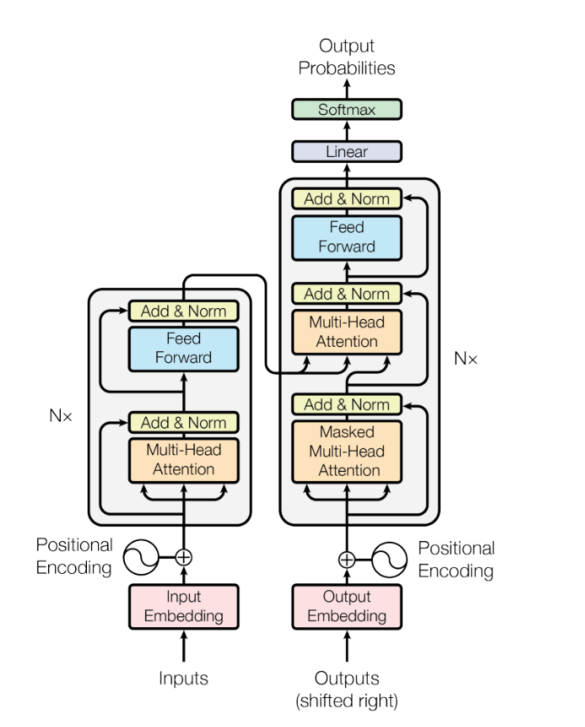
\includegraphics[width=0.7\textwidth]{fig1.png}
\caption{Figure 1: Schematic diagram of the Transformer architecture model}
\end{figure}

\begin{figure}[H]
\centering
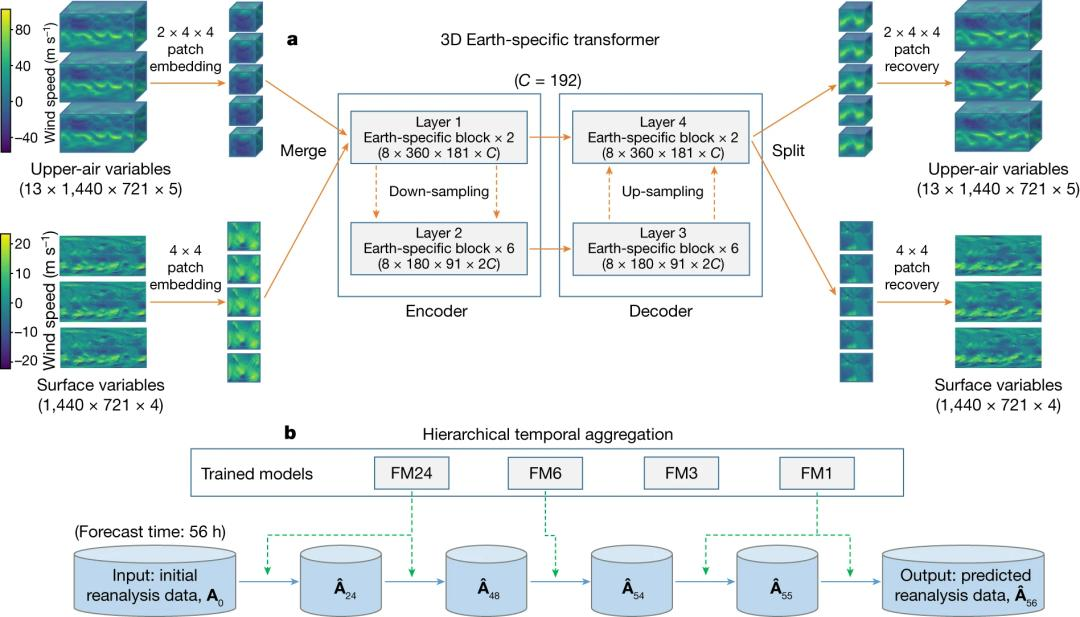
\includegraphics[width=0.7\textwidth]{fig2.jpg}
\caption{Figure 2: Schematic diagram of the Pangu Weather model}
\end{figure}

\section{Feeling: Why This Lecture Left Such a Deep Impression}

This lecture left a deep impression on me for roughly three reasons.

The first reason is that the topic aligned well with my own knowledge background. In high school, I taught myself Python programming and was exposed to some basic machine learning concepts such as convolutional neural networks and backpropagation. Although I had no formal competition or project experience, I have always been interested in computers and algorithms. After entering the atmospheric science major, I was confused for a while about how to combine these two interests. This lecture clearly demonstrated the intersection of AI and atmospheric science—smart meteorology or AI meteorology—pointing me toward a concrete and viable direction.

The second reason is the instructor's clear and straightforward communication style. He neither avoided technical details nor deliberately used obscure jargon to create distance. For example, when explaining the Pangu model, he directly showed the model's network structure diagram and explained why the self-attention mechanism in Transformers is well-suited for processing atmospheric data—namely, because of the long-range dependencies between different regions of the atmosphere. This approach of explaining the principles while providing intuitive understanding allowed me, despite my limited professional knowledge, to grasp the core ideas.

The third reason is the strong real-world impact of the lecture's content. When the instructor compared the computational energy consumption of traditional numerical models with AI models, I suddenly realized that AI is not just about faster computation—it could fundamentally change the engineering paradigm of weather forecasting. A forecasting system that can run on a single server means that developing countries, remote areas, and even individual researchers could gain access to forecasting capabilities that were previously only affordable to top meteorological centers \cite{Bauer2015Quiet}. The equity improvement brought by this technology strikes me as having significant social value.

\section{Reflection: Knowledge Points and Ideas That Sparked My Interest and Thinking}

Several ideas from the lecture sparked my interest and prompted further reflection, leading me to look up additional information after class.

The first is whether AI can replace physical parameterization schemes in numerical models \cite{Schneider2017Earth}. In traditional numerical models, sub-grid processes such as cumulus convection and boundary layer turbulence must be approximated using parameterization schemes, which themselves carry many empirical assumptions. The instructor mentioned that some research is attempting to use neural networks to directly learn the mapping between sub-grid fluxes and grid-scale variables, thereby replacing traditional parameterization schemes \cite{Brenowitz2018Prognostic}. This made me think about two aspects: on one hand, could purely data-driven parameterization schemes violate basic physical conservation laws? On the other hand, if the training data comes from high-resolution cloud-resolving models, the physics learned by the AI is merely another numerical approximation rather than real atmospheric processes. This question does not seem easy to answer.

The second is the problem of few-shot learning for extreme weather \cite{Gagne2014Machine}. The lecture mentioned that for rare weather events such as typhoons, tornadoes, and extreme rainfall, there are very few historical samples available for training, which leads to poor performance of AI models when encountering extreme situations. The instructor gave an example of an AI model that performed well for routine precipitation forecasts but significantly underestimated rainfall during a once-in-a-century heavy rain event. This reminded me of the out-of-distribution generalization problem in machine learning: when the training set and test set have different distributions, model performance degrades sharply. Teaching AI to handle unseen situations may require incorporating physical constraints, data augmentation, or meta-learning methods. I find this direction challenging and highly valuable for research.

The third is the problem of interpretability in AI forecasts \cite{Ham2020Deep}. Although traditional numerical models are complex, each step follows physical equations, allowing forecasters to trace errors back to their sources. However, the black-box nature of deep learning makes it difficult for forecasters to understand the basis for an AI forecast conclusion. The instructor said the current trend is toward explainable AI, such as using attention maps or feature visualization to show forecasters which areas the model focuses on \cite{Tjoa2020Survey}. However, whether such methods can provide reliable physical explanations remains controversial. I personally believe that if AI is to become a trustworthy tool in forecasting decisions rather than merely a black-box reference, explainability must be fundamentally addressed.

\section{Exploration: Investigation and Understanding of a Specific Research Direction}

Given the reflections above, I chose the direction of AI meteorology for a more detailed investigation. Below is my understanding of this direction, formed after consulting various sources.

\subsection{Main Research Areas}

The research scope of AI meteorology is quite broad, with several currently active sub-directions.

The first is radar echo extrapolation and short-term nowcasting, using recurrent neural networks, convolutional LSTM, or attention-based models to predict how radar reflectivity factor images will evolve over the next zero to six hours based on past few hours of data \cite{Shi2015Convolutional}. Compared with traditional optical flow methods, deep learning approaches better capture nonlinear processes such as the genesis, merger, and splitting of convective cells.

The second is AI post-processing of numerical forecasts. Traditional post-processing methods include model output statistics and ensemble calibration. In recent years, researchers have begun using random forests, gradient boosting, or small-scale neural networks to perform bias correction and probabilistic forecasting on numerical model outputs \cite{Rasp2018Deep}, significantly improving the forecast accuracy of variables such as precipitation and wind speed.

The third is large-scale weather models, including Pangu Weather \cite{Bi2022}, GraphCast \cite{Lam2023}, and FourCastNet \cite{Pathak2022FourCastNet}. These models are pre-trained on large reanalysis datasets using Transformer or graph neural network architectures, achieving comparable or even better medium-range forecast performance than traditional numerical models. Their advantage is high computational efficiency, but their disadvantage is the difficulty of incorporating real-time observational data; they are currently used in a post-processing manner.

The fourth is physics-guided machine learning \cite{Kashinath2021Physics}. To prevent purely data-driven models from violating physical laws, researchers attempt to embed governing equations—such as the Navier-Stokes equations—as constraints or loss functions into the neural network training process. This approach maintains physical consistency while preserving computational efficiency.

\subsection{Social Significance}

The social significance of AI meteorology can be understood at two levels. From a disaster prevention and mitigation perspective, faster forecast speeds and higher accuracy mean earlier warnings and better preparedness. For example, increasing the lead time for severe convection warnings from the current twenty to forty minutes to over sixty minutes should significantly reduce casualties and property losses. From an inclusive service perspective, the low computational cost of AI models means that high-quality forecasts are no longer accessible only to developed countries with supercomputers \cite{WMO2021Smart}. For regions such as Africa and Southeast Asia, where meteorological observations and computing resources are relatively scarce, this has considerable practical significance.

\subsection{Development Prospects}

Looking at current trends, AI meteorology is likely to evolve toward a hybrid paradigm in the next five to ten years. In this paradigm, numerical models provide physically consistent background fields, while AI modules rapidly generate fine-grained forecasts for specific variables or perform intelligent corrections of numerical model outputs. Meanwhile, end-to-end pure AI forecast models will continue to advance, but they are unlikely to completely replace numerical models in the short term, particularly in areas such as extreme events and long-term climate prediction \cite{Schultz2021Can}.

I believe that interpretability, uncertainty quantification, and real-time data assimilation will be the three bottlenecks that AI meteorology needs to overcome in the next stage. Resolving these issues will allow AI meteorology to transform from a laboratory toy into an operational tool.

\begin{figure}[H]
\centering
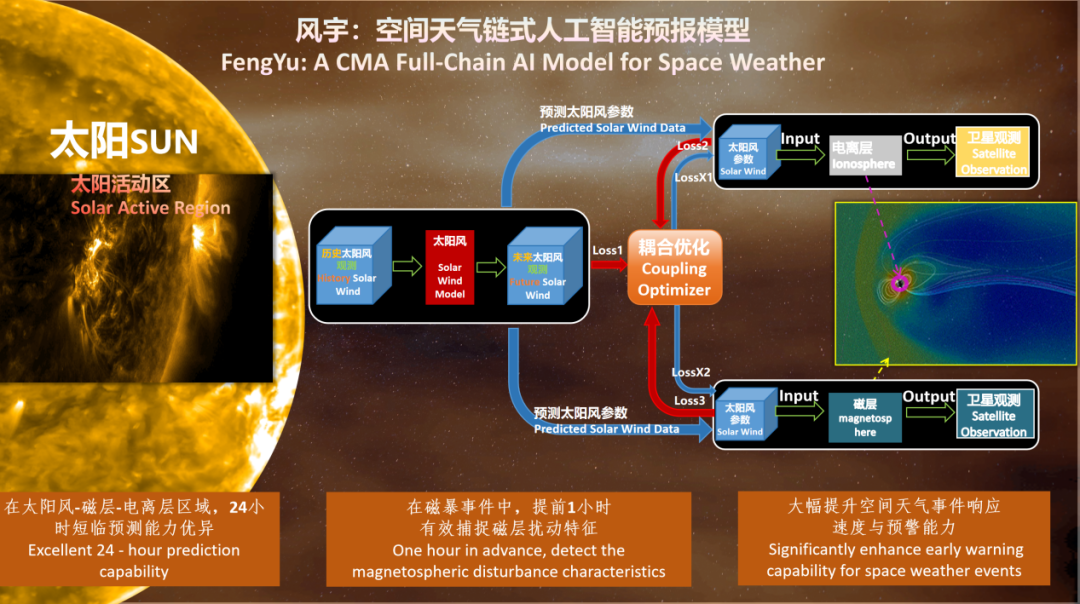
\includegraphics[width=0.4\textwidth]{fig3.png}
\caption{Figure 3: Schematic diagram of the Fengyu model}
\end{figure}
\begin{figure}[H]
\centering
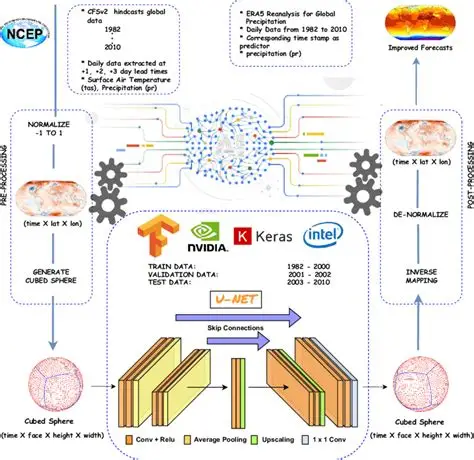
\includegraphics[width=0.4\textwidth]{fig4.png}
\caption{Figure 4: Schematic diagram of NCEP}
\end{figure}

\section{Choice: My Interest in This Direction and Potential Future Decisions}

After attending this lecture and conducting further research, I have developed a clear interest in the interdisciplinary direction of AI meteorology and have tentatively identified it as a possible path for my future professional development.

The source of my interest is twofold. First, it lies precisely at the intersection of my existing knowledge and my future learning goals. I have some programming foundation and have always been interested in machine learning, while my atmospheric science courses are gradually helping me build an understanding of the physical mechanisms of weather and climate. AI meteorology requires competence in both areas, which makes me feel that I am not starting from scratch but rather from a relatively advantageous position. Second, this direction has both theoretical depth and practical application value. The nonlinear, multi-scale, and chaotic nature of the atmospheric system provides a challenging application scenario for machine learning research. At the same time, the成果 of AI meteorology can directly translate into disaster prevention and mitigation benefits. This sense of learning something that can be used to make a difference is something I value highly.

Regarding my future plan, my current thinking is as follows. At the undergraduate level, I need to strengthen three foundational areas simultaneously. The first is core atmospheric science courses, particularly dynamic meteorology, synoptic meteorology, radar meteorology, and cloud physics. The second is mathematics and statistics foundations, including probability theory, mathematical statistics, and time series analysis. The third is computer and data science skills, such as Python programming, PyTorch or TensorFlow frameworks, and basic machine learning algorithms. I plan to try joining a research group working on AI meteorology within my college during my sophomore or junior year, to participate in some relatively simple research training projects—such as building a small-scale radar echo extrapolation model or assisting with the cleaning and labeling of meteorological datasets. These experiences will help me more concretely assess whether I am truly suited for this direction.

After graduation, I am currently leaning toward continuing on to graduate school to conduct in-depth research on a specific problem in AI meteorology, such as few-shot learning for extreme weather, physics-constrained neural networks, or the application of AI in data assimilation \cite{Geer2020Machine}. My ultimate goal is to enter a meteorological operational agency or research institution, working on the development and operational application of AI meteorological models.

I am also fully aware that this direction still has many unresolved issues—interpretability, generalization capability, and physical consistency, among others. But it is precisely these challenges that make the research valuable. A field that is difficult but still growing may be just right for someone willing to grapple with both physics and code.

\begin{thebibliography}{99}

\bibitem{Chen2004Numerical}
Chen D.H., Xue J.S. Current status and prospects of operational numerical weather prediction models[J]. Acta Meteorologica Sinica, 2004, 62(5): 623-633.

\bibitem{Lecun2015Deep}
LeCun Y., Bengio Y., Hinton G. Deep learning[J]. Nature, 2015, 521(7553): 436-444.

\bibitem{Shi2015Convolutional}
Shi X., Chen Z., Wang H., et al. Convolutional LSTM network: A machine learning approach for precipitation nowcasting[C]. Advances in Neural Information Processing Systems, 2015: 802-810.

\bibitem{Reichstein2019Deep}
Reichstein M., Camps-Valls G., Stevens B., et al. Deep learning and process understanding for data-driven Earth system science[J]. Nature, 2019, 566(7743): 195-204.

\bibitem{Bi2022}
Bi K., Xie L., Zhang H., et al. Pangu-Weather: A 3D high-resolution model for fast and accurate global weather forecast[J]. arXiv preprint arXiv:2211.02556, 2022.

\bibitem{McGovern2019Making}
McGovern A., Lagerquist R., Gagne D.J., et al. Making the black box more transparent: Understanding the physical implications of machine learning[J]. Bulletin of the American Meteorological Society, 2019, 100(11): 2175-2199.

\bibitem{Bauer2015Quiet}
Bauer P., Thorpe A., Brunet G. The quiet revolution of numerical weather prediction[J]. Nature, 2015, 525(7567): 47-55.

\bibitem{Schneider2017Earth}
Schneider T., Lan S., Stuart A., et al. Earth system modeling 2.0: A blueprint for models that learn from observations and targeted high-resolution simulations[J]. Geophysical Research Letters, 2017, 44(24): 12396-12417.

\bibitem{Brenowitz2018Prognostic}
Brenowitz N.D., Bretherton C.S. Prognostic validation of a neural network unified physics parameterization[J]. Geophysical Research Letters, 2018, 45(12): 6289-6298.

\bibitem{Gagne2014Machine}
Gagne D.J., McGovern A., Xue M. Machine learning enhancement of storm-scale ensemble probabilistic quantitative precipitation forecasts[C]. 27th Conference on Severe Local Storms, 2014.

\bibitem{Ham2020Deep}
Ham Y.G., Kim J.H., Luo J.J. Deep learning for multi-year ENSO forecasts[J]. Nature, 2020, 573(7775): 568-572.

\bibitem{Tjoa2020Survey}
Tjoa E., Guan C. A survey on explainable artificial intelligence (XAI): Toward medical XAI[J]. IEEE Transactions on Neural Networks and Learning Systems, 2020, 32(11): 4793-4813.

\bibitem{Rasp2018Deep}
Rasp S., Leroux S. Deep learning for post-processing ensemble weather forecasts[J]. arXiv preprint arXiv:1805.09091, 2018.

\bibitem{Lam2023}
Lam R., Sanchez-Gonzalez A., Willson M., et al. GraphCast: Learning skillful medium-range global weather forecasting[J]. Science, 2023, 382(6677): 1416-1421.

\bibitem{Pathak2022FourCastNet}
Pathak J., Subramanian S., Harrington P., et al. FourCastNet: A global data-driven high-resolution weather model using adaptive Fourier neural operators[J]. arXiv preprint arXiv:2202.11214, 2022.

\bibitem{Kashinath2021Physics}
Kashinath K., Mustafa M., Albert A., et al. Physics-aware machine learning for Earth science[J]. AGU Fall Meeting Abstracts, 2021.

\bibitem{Schultz2021Can}
Schultz M.G., Betancourt C., Gong B., et al. Can deep learning beat numerical weather prediction?[J]. Philosophical Transactions of the Royal Society A, 2021, 379(2194): 20200097.

\bibitem{WMO2021Smart}
World Meteorological Organization (WMO). Smart Meteorology and AI Applications Report[R]. Geneva: WMO, 2021.

\bibitem{Geer2020Machine}
Geer A.J. Learning earth system models from observations: machine learning for data assimilation[J]. ECMWF Technical Memorandum, 2020, 876.

\end{thebibliography}

\end{document}